%--------------------------------------------------------------------
%--------------------------------------------------------------------
% Formato para los talleres del curso de Herramientas Computacionales
% Universidad de los Andes
%--------------------------------------------------------------------
%--------------------------------------------------------------------

\documentclass[11pt,letterpaper]{exam}
\usepackage[utf8]{inputenc}
\usepackage[spanish]{babel}
\usepackage{graphicx}
\usepackage{mdframed}
\usepackage{tabularx}
\usepackage[absolute]{textpos} % Para poner una imagen completa en la portada
\usepackage{multirow}
\mdfdefinestyle{mystyle}{leftmargin=1cm,rightmargin=1cm,linecolor=red}
\usepackage{float}
\usepackage{hyperref}
\usepackage{xcolor}
\decimalpoint
\hypersetup{colorlinks=false,linkbordercolor=red,linkcolor=green,pdfborderstyle={/S/U/W 1}}

%\usepackage{pst-barcode}
%\usepackage{auto-pst-pdf}

\newcommand{\base}[1]{\underline{\hspace{#1}}}
\boxedpoints
\pointname{ pt}
%\extrawidth{0.75in}
%\extrafootheight{-0.5in}
\extraheadheight{-0.15in}
%\pagestyle{head}

%\noprintanswers
%\printanswers
\renewcommand{\solutiontitle}{}
\SolutionEmphasis{\color{blue}}

\usepackage{upquote,textcomp}
\newcommand\upquote[1]{\textquotesingle#1\textquotesingle} % To fix straight quotes in verbatim

\begin{document}
\begin{center}
{\Large Herramientas Computacionales} \\
Taller 10 - \textsc{Python}: herramientas estadísticas (2) \\
{\small \it Abril de 2015}
\end{center}

\begin{textblock*}{40mm}(10mm,20mm)
  
\includegraphics[width=3cm]{logoUniandes.pdf}
\end{textblock*}

\begin{textblock*}{40mm}(161mm,20mm)
  
\includegraphics[width=3cm]{logoUniandes.pdf}
\end{textblock*}

\vspace{1cm}

La solución de este taller debe ser presentada en un solo archivo comprimido con nombre \verb+NombreApellido_HW10.zip+. El archivo comprimido debe tener el script del primer literal y un cuaderno de \verb+iPython+ con las otras respuestas. Puede trabajarse en grupo de máximo tres estudiantes.

\begin{center}
	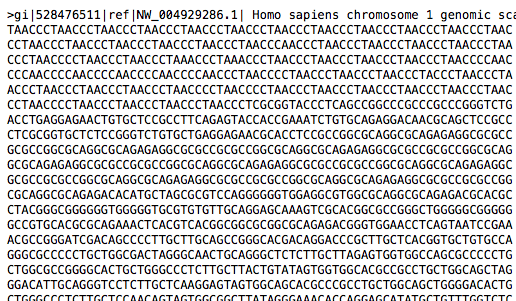
\includegraphics[width=0.7\textwidth]{./cromo.png}
\end{center}

\begin{questions}

\question
\begin{parts}
	\part[25] Escriba un script de \verb+Bash+ con nombre \verb+downbot.sh+ que descargue y descomprima de forma programática los 22 autosomas del genoma humano (los archivos \verb+.fa.gz+). Los archivos están alojados en un servidor FTP del NCBI en directorios encontrados en \href{ftp://ftp.ncbi.nih.gov/genomes/Homo_sapiens/}{ftp://ftp.ncbi.nih.gov/genomes/Homo\_sapiens/}, y cuando se descomprimen el resultado son archivos de texto de tipo  \href{http://en.wikipedia.org/wiki/FASTA_format}{FASTA}. Explore la estructura de los archivos. El script debe tener menos de $300$ caracteres. Para descomprimir los archivos el comando \verb+gunzip+ puede ser de utilidad.
	
PRECAUCIÓN: tenga en cuenta que la cantidad de información a descargar es de aproximadamente $1$GB.
	
%Adenina: 789545480
%Timina: 790577982
%Citosina: 548794799
%Guanina: 549028262


	\part[25] Escriba código en \verb+Python+ que cuente el total de $A$, $G$, $T$, y $C$ en el conjunto de todos los autosomas. Tenga cuidado de no procesar el encabezado de los archivos.
	\part[25] Escriba código en \verb+Python+ que cuente y guarde en cuatro listas \verb+countA+, \verb+countG+, \verb+countT+ y \verb+countC+ la cantidad de ocurrencias de cada base nitrogenada en las líneas de los archivos de los autosomas (cada una con $70$ caracteres).  Tenga cuidado de no procesar el encabezado de los archivos. Calcule el promedio, mediana y desviación estándar de cada lista.
	\part[25]  Haga tres histogramas cumulativos: uno que incluya en los mismos ejes los histogramas de \verb+countG+ y \verb+countC+, los de \verb+countA+ y \verb+countT+, y los de \verb+countG+ y \verb+countA+. Todos los histogramas deben tener leyendas apropiadas y estar normalizados. Los resultados deben ser similares a lo mostrado en la siguiente figura y deben estar incluidos en el cuaderno de \verb+iPython+.
\end{parts}

\begin{center}
	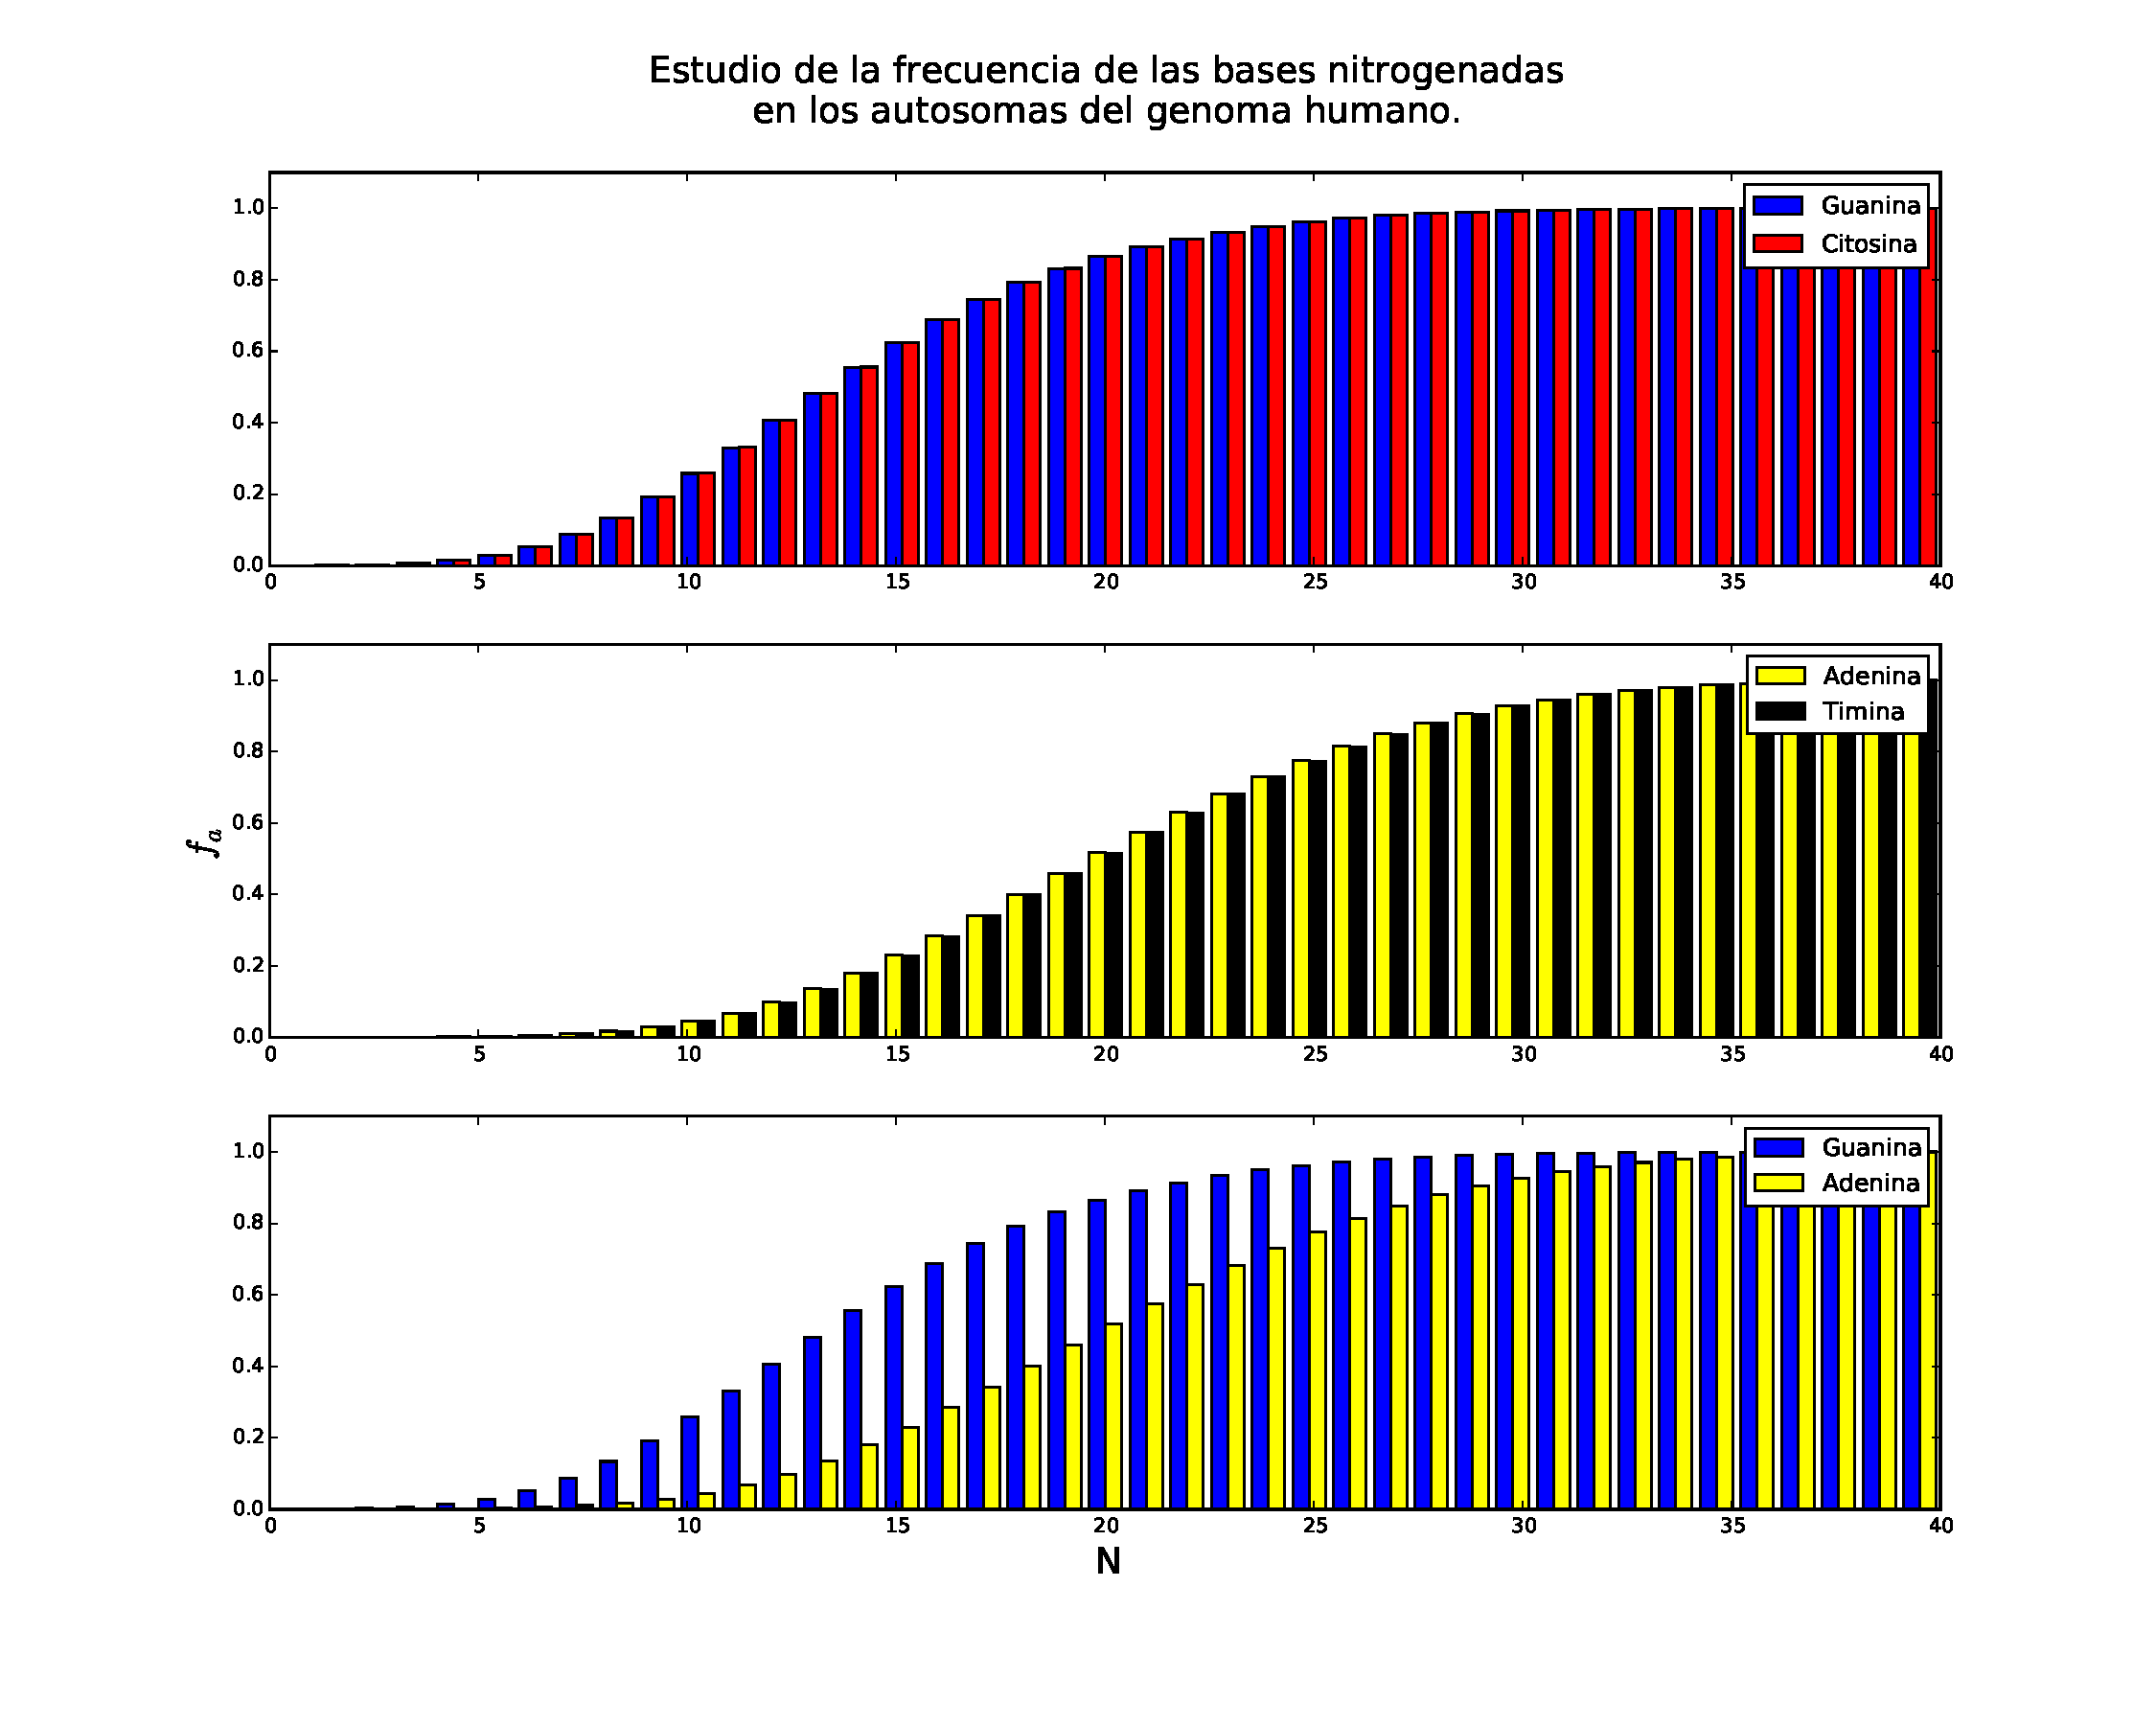
\includegraphics[width=0.99\textwidth]{./bases.pdf}
\end{center}
\end{questions}
\end{document}
